\section{Approach}
\label{sec:approach}

%In this section, we describe the model architecture used for our experiments
%and propose our reducing repetition method which is implemented by extending thebasic model.
%and propose our novel repetition reduction method, which is an extension to the basic model.
%~\footnote{
%All of the data and source code
%can be downloaded from http://Anonymous.}

In summarization task, the input (source document) and
output (summary) are both sequences of words.
Suppose the input and output are respectively represented as
$\textbf{x} = (x_{1},x_{2},...,x_{m})$ and 
$\textbf{y} = (y_{1}, y_{2},..., y_{n})$ ($m>n$),
the goal is to maximize the conditional probability
$p(\textbf{y} | \textbf{x}) \!=\! {\prod^n_{t} {p(y_{t} | y_{1}, y_{2},..., y_{t-1}, \textbf{x}})}$.

%We aim to generate summaries that are not only fluent 
%and logically consistent with source document, but also with 
%a small amount of repeatedness, which is natural in human written summaries.  
\subsection{Basic CNN seq2seq Model}
\label{sec:basic}
Our basic model is multi-layer CNN seq2seq networks \cite{gehring2017convs2s} with attention mechanism
\footnote{\url{https://github.com/facebookresearch/fairseq-py}}.
%as illustrated in \figref{fig:basicModel}. 
%\begin{figure}[th]
%    \centering
%    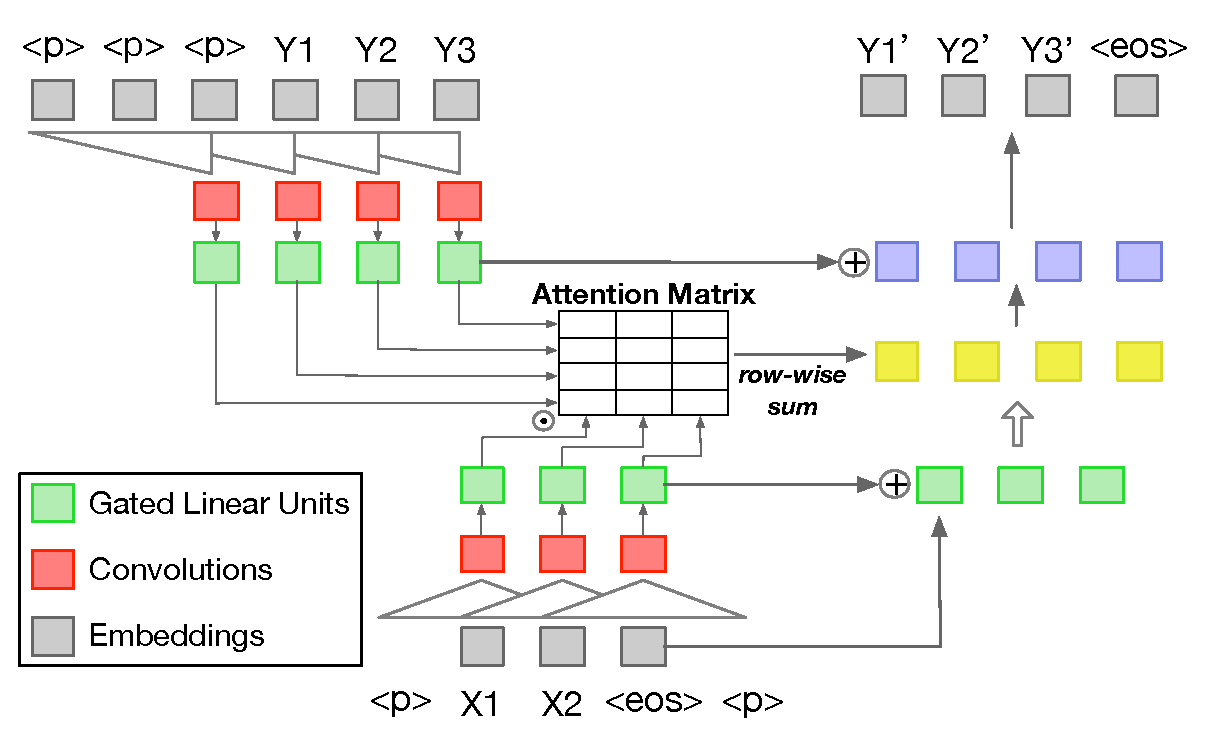
\includegraphics[width=0.5\linewidth]{cnn}
%    \caption{Convolutional seq2seq model.}
%	%$\odot$ stands for inner product. $\oplus$ stands for element-wise addition.}
%    \label{fig:basicModel}
%\end{figure}
We combine word embeddings and position embeddings to obtain input $\mathbf{X} = (X_1,...,X_m)$ and output $\mathbf{Y}=(Y_1,...,Y_n)$. 
%We denote $\mathbf { z } ^ { l }$ and $\mathbf { h } ^ { l }$ 
We denote $\mathbf { z } ^ { l } = \left( z _ { 1 } ^ { l } , \ldots , z _ { m     } ^ { l } \right)$ and $\mathbf { h } ^ { l } = \left( h _ { 1 } ^ { l } , \ldots , h _ { n } ^ { l } \right)$ 
respectively as convolutional output of the encoder and
decoder in the $l$-th layer.
%where $\mathbf { z } ^ { l } = \left( z _ { 1 } ^ { l } , \ldots , z _ { m } ^ { l } \right)$ and $\mathbf { h } ^ { l } = \left( h _ { 1 } ^ { l } , \ldots , h _ { n } ^ { l } \right)$. 
Each element of the output
sequence generated by the decoder network is fed
back into the next layer of decoder network.
In each layer, GLU \cite{DauphinFAG17} and residual connections \cite{HeZRS16}
are used respectively as a non-linear gate and guarantee for sufficient depth of the network.  
\begin{equation}
\small
    h _ { i } ^ { l } = GLU \left( W ^ { l } \left[ h _ {i-k/2 } ^ { l - 1 } , \ldots , h _ { i+k/2 } ^ { l - 1 } \right] + b _ { w } ^ { l } \right) + h _ { i } ^ { l - 1 }
\end{equation} 
where \textit{k} is kernel width. $W$ and $b$ are trainable parameters.
Next, we compute the probability distribution for the next word
using the top decoder output:
\begin{equation}
\small
    p \left( y _ { i + 1 } | y _ { 1 } , \ldots , y _ { i } , \mathbf { x } \right) = \operatorname { softmax } \left( W _ { o } h _ { i } ^ { L } + b _ { o } \right)
\end{equation}

For each decoder layer,
we compute decoder state $d_{i}^{l}$ for attention via
\begin{small}
\begin{align}
\label{eq:a}
    d _ { i } ^ { l } = W _ { d } ^ { l } h _ { i } ^ { l } + b _ { d } ^ { l } + Y _ { i } \quad \quad
    a _ { i j } ^ { l } = \frac { \exp \left( d _ { i } ^ { l } \cdot z _ { j } ^ { u } \right) } { \sum _ { t = 1 } ^ { m } \exp \left( d _ { i } ^ { l } \cdot z _ { t } ^ { u } \right) } \quad \quad
    c _ { i } ^ { l } = \sum _ { j = 1 } ^ { m } a _ { i j } ^ { l } \left( z _ { j } ^ { u } + X_j \right) 
\end{align}
\end{small}
%where $z_{j}^{u}$ is the encoder output of last layer $u$.  
where $d_{i}^{l}$ is decoder state, $z_{j}^{u}$ is the encoder state, 
$u$ is the last layer of encoder
and $a_{ij}$ is attention score.
Finally, $c _ { i } ^ { l }$ 
is the weighted sum of encoder states and input representations,
which is added to $h_{i}^{l}$ and forms the input for the next decoder layer or the final output.


\subsection{Attention Filter Mechanism (ATTF)}
\label{sec:attf}
%We propose an attention filter mechanism based on basic model
We propose an attention filter mechanism as a novel extension 
to the basic model,
which can record previously attended locations 
%previously POIs 
in the source document directly and generate summaries 
%without repetition
with a natural level of repeatedness. 
This method aims at relieving the repetition problem caused by 
decoders attending to the same POI in source document.

\begin{figure}[th!]
\centering
\subfigure[Attention Filter Mechanism (ATTF)]{
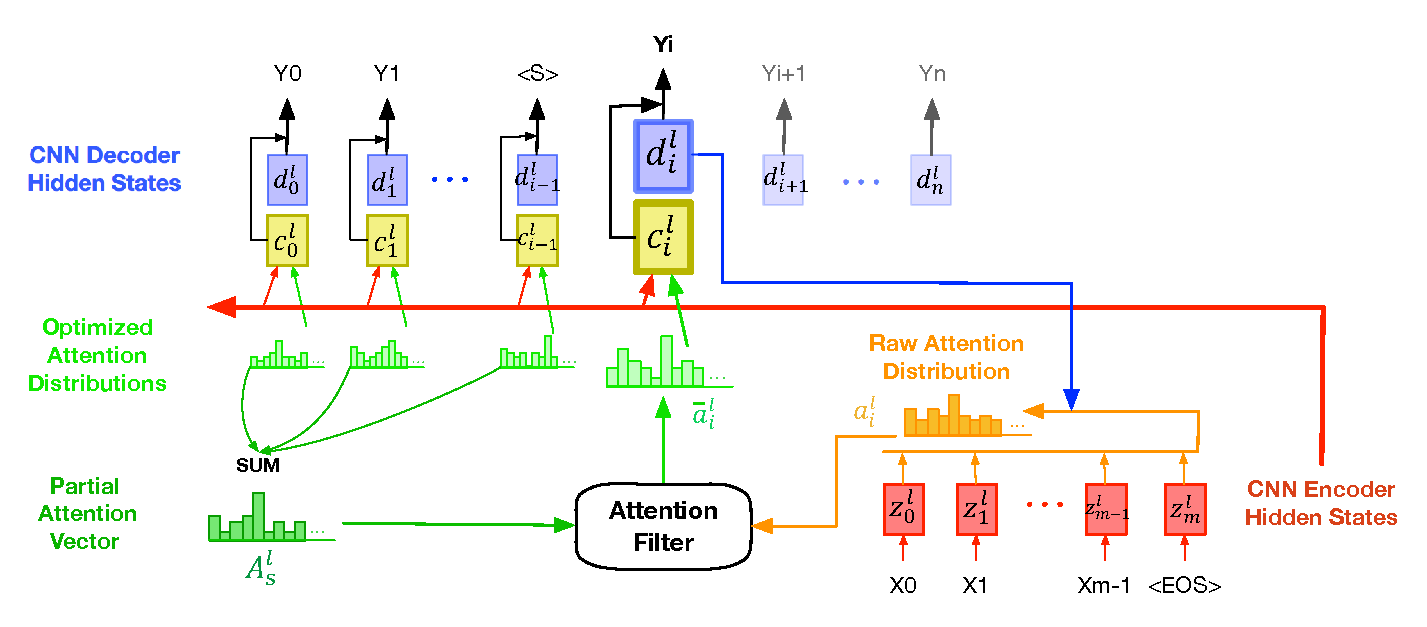
\includegraphics[width=0.5\linewidth]{model}
}
\quad
\subfigure[Sentence-level Backtracking Decoder (SBD)]{
\includegraphics[width=0.4\linewidth]{SBD}
}
\caption{Overview of ATTF and SBD. (a) shows ATTF.
	    (b) is SBD (beam size = 3), which shows the progress of generating summary at test. The circles denote the
		candidate words (choices) in vocabulary, 
		which are sorted by the probability of being selected in
		descending order. Each circle at level $l$ has $N$ choices 
		at level $l+1$. $N$ is the number of words in vocabulary. 
		The number in circles is the order of these choices according to the
		probability. The generation order is from level 1 (top) to level 3 (bottom).}
\label{fig:model_main}
\end{figure}

%\begin{figure}[th]
%	\centering
%	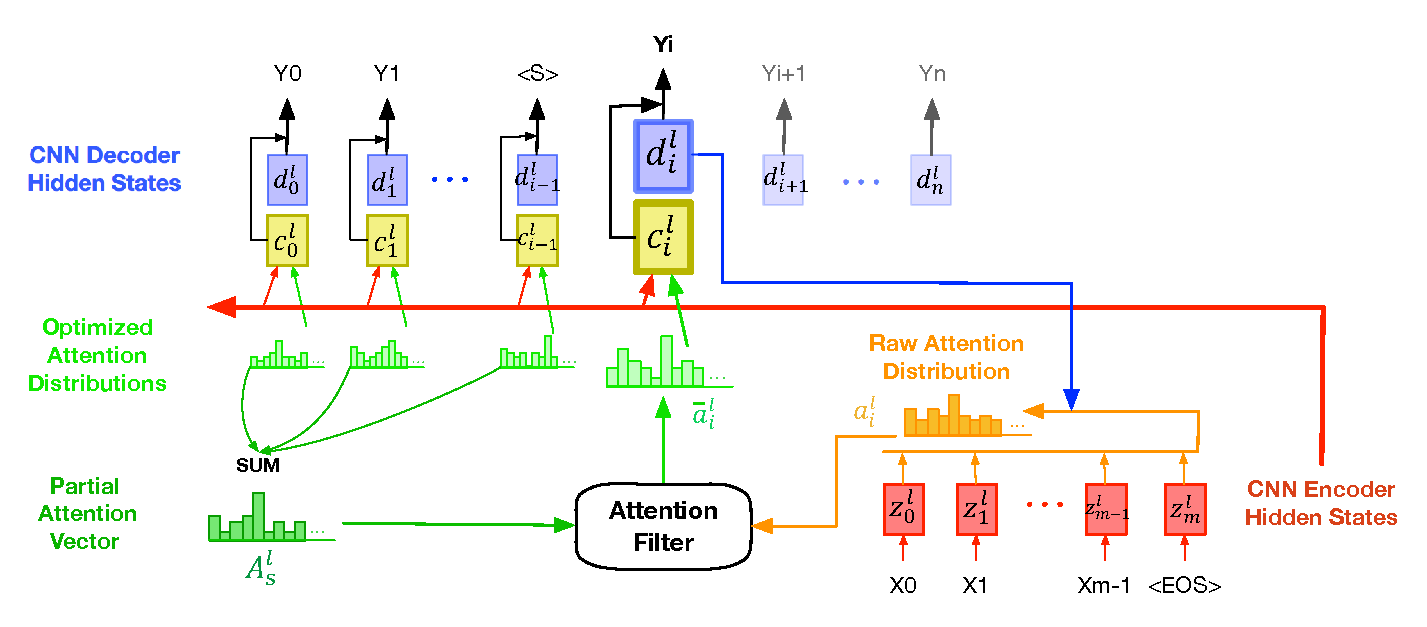
\epsfig{file=model, width=0.8\columnwidth}
	%\caption{Overview of proposed model, which shows how Attention Filter Mechanism (ATTF) works when decoding $Y_i$.}
%	\caption{Overview of Attention Filter Mechanism (ATTF)}
%	\label{fig:model_main}
%\end{figure}

In this mechanism, both source document and summary are 
respectively split into 
\textit{sections} and \textit{segments} by punctuations. We
denote the punctuation marks as \verb#<S>#.
$\mathbf{u}=(u_{0},u_{1},...,u_{M})$ 
and $\mathbf{v}=(v_{0},v_{1},...,v_{N})$
denote the positions of \verb#<S># in source document and summary.
Both $u_{0}$ and $v_{0}$ are $-1$.
%Source document $\mathbf{U}=(U_{0},U_{1},...,U_{M-1})$ 
%and summary $\mathbf{V}=(V_{0},V_{1},...,V_{N-1})$ are represented in the form of sections and.
Therefore, we can represent source document as $\mathbf{U}=(U_{0},U_{1},...,U_{M-1})$ in the form of \textit{sections}. Similarly, for summaries, we have $\mathbf{V}=(V_{0},V_{1},...,V_{N-1})$. 
$U_i$ and $V_i$ are
both sequence of tokens minus the punctuation tokens.
%\KW{They are all substrings splitted by punctuations.}

Let $D$ denote the number of tokens in the source document.
We define \textit{segment attention vector} in the $l$-th layer as 
$A^{l} = (A_{0}^{l}, A_{1}^{l},..., A_{N}^{l})$, 
where $A_s^l\subset \mathbb{R}^{D}$ is a vector representing 
segment attention distribution, of the $s$-th \textit{segment},
over tokens in the source document. Summing up attention score vectors 
of each position in the $s$-th \textit{segment}:
$A_{s}^{l} = \sum_{i=v_{s-1}+1}^{v_{s}-1}a_{i}^{l}$ where
$a_i^l$ is also a $D$-dimensional vector that records 
the attention scores of the $i$-th token in the summary over 
tokens in the source document. In other words, $ A_{s}^{l}$ 
measures the relevance between tokens of the source document and 
the $s$-th \textit{segment} $V_s$. 
%where vector $A_{n}^{l}$ is the partial attention distribution over the words in source document. 
%It represents the degree of relevance between source document and the $n$-th section in summary.
We set $A_{0}^{l}$ as zero vector, because nothing is attended before generating 
the first \textit{segment}. 


To find the most attended \textit{sections}, 
we sort the elements inside the filter vector, 
$A_{s}^{l}$, in descending order, 
and record the top $k$ elements' positions in 
the source document as $\mathbf{p}=(p_{0},...,p_{k})$ where
$k=v_{s}-v_{s-1}-1$.
%To get the attended sections of document, we sort elements $A_{nj}^{l}$ in descending order, and record the positions a
%in decreasing order, and record the position
%$\mathbf{p}=(p_{0},...,p_{k})$, of 
%top $k$ elements in source document, where $k = v_{n} - v_{n-1}$. 
%The higher value of $A_{nj}^{l}$ means that the $j$-th words of source document has been attended. 
%We find out which section of these top $k$ elements belong to by $\mathbf{p}$ and $\mathbf{u}$.
Next, we locate these elements in the source document as well as
the \textit{sections} they belong to. 
We assign each section a set of positions that have been attended to, 
$P_{U_{t}}$. 
If the size of $P_{U_{t}}$ is larger than
$sz$, a predefined constant,
%\footnote{$sz$ is a constant. 
%We set $sz$ as 3, because nearly 90 percent
%of sections with lengt$>=$3.}, 
the \textit{section} $U_{t}$ should not be attended again. 
That is, $U_{t}$ is a POI of segment $V_{s}$.
%We use $\bar{U}$ to express this kind of section. 
$\mathbb{U}_{s}$ denotes a set of all such POIs for $V_s$.
$\mathbb{U}_{0}$ is an empty set.
%the \textit{section $U_{t}$} can be seen as the POI by $V_s^{l}$. 

We construct two multi-hot vectors $g_{s}$ and $g'_{s}$ for each \textit{segment} $V_{s}$.
The dimensions of them are the
same as $A_{s}^{l}$. For $g_{s}$, we set elements on the position of tokens
belonging to sections in $\mathbb{U}_{s}$ to 0, and other
%same as $A_{s}^{l}$. For $g_{s}$, we set elements on the position of POIs to 0, and other
positions to 1. $g'_{s}$ is the flipped version of $g_{s}$. 
%The filter on $a_{ij}^{l}$ in Equation (\ref{eq:a} is to minimize elements of POIs:
The filtered $a_{ij}^{l}$ and $c$ in Equation (\ref{eq:a}) now becomes:
%\begin{equation}
%\small
%    e_{s} = \min \limits_{A_{s}}\left(\frac{A_{sj}^{l}}{v_{s}-v_{s-1}-1}\right)
%\end{equation}
%\begin{equation}
%\small
%    \tilde{a}_{ij}^{l} = a_{ij}^{l}\prod_{q=0}^{s}g_{qj} + e_{s}g_{sj}'
%    %\bar{a_{ij}}^{l} = a_{ij}^{l}\prod_{q=0}^{n}s_{q} + \min\frac{A_{n}^{l}}{v_{n}-v_{n-1}}t_{n}
%\end{equation}
\begin{small}
\begin{align}
	\tilde{a}_{ij}^{l} = a_{ij}^{l}\prod_{q=0}^{s}g_{qj} + \min \limits_{A_{s}}\left(\frac{A_{sj}^{l}}{v_{s}-v_{s-1}-1}\right)g_{sj}' \quad \quad
    c _ { i } ^ { l } = \sum _ { j = 1 } ^ { m } \tilde{a}_{ij}^{l} \left( z _ { j } ^ { u } + X_j \right)
\end{align}
\end{small}
where $v_{s}$ is the maximum value in 
$\mathbf{v}$ that is smaller than $i$, and $\tilde{a}_{ij}^l$ is the filtered
attention score. $A_{sj}$ is the attention score between $j$-th token
of the source document and the $s$-th \textit{segment}. 
$g_{sj}$ and $g_{sj}'$ denote whether $j$-th token
of the source document has been attended.
%\XS{Hard to understand this definition of ``n''. And ``n'' is already used to be the size of output in Section 2.1}

%We pick $K$ sections with highest attention which is calculated by:
%\begin{equation}
%    A_{nj}^{l} = \sum^{P}A_{nj}^{l}
%\end{equation}  

%This method find out the attended location in source document directly and accurately.
%Then it filters out attention of the attended location from the attention distribution. 
%%In this way, our attention filter is capable of comprehending the attention history in a precise and direct manner. 
%The previous approaches revise attention scores
%through decoder hidden state. They can not locate POIs exactly.
%The coverage model which gets the sum of all previous attention can 
%bring attention noise, especially in the long summary.

%Because of using segment attention and revising attention score of attended POIs directly,
By using segment-wise attention and revising attention scores of attended POIs directly,
%it optimizes the 
%\KW{compared with token-wise attention,}
our model optimizes the
attention distribution between encoder states and decoder states in such a way that
the alignment relationship between source document and summary is enhanced, 
and noise for attention from encoder outputs is reduced. 
\cut{%%%%%%%%%%%%
As shown in \tabref{tab:attn_exp}, %the segments in example are separated by punctuation.
for basic CNN model, the 2nd and 3rd sentence repeatedly attend to 
the 5th segment in source.
After applying ATTF model, 
the attention score of 3rd and 5th segment in source are penalized 
during generating words in 3rd sentence of ATTF.
The last sentence of the summary generated by ATTF attend to 7th segment in source.

\begin{table}[th!]
\scriptsize
\begin{center}
\caption{\label{tab:attn_exp} Summary generated by the basic CNN model and ATTF model}
\begin{tabular}{|l|l|}%{|p{7cm}|rl|}
\hline 
\multicolumn{2}{|c|}{\bf Source document} \\
\hline
\multicolumn{2}{|c|}{\tabincell{l}{(1)justin timberlake and jessica biel, (2)welcome to parenthood. 
	   (3)the celebrity couple announced the arrival of their son, \\
       (4)...(5)the couple announced the pregnancy in january, (6)...  
	   (7)it is the first baby for both . }} \\
\hline 
\bf Basic CNN model (CNN) & \bf ATTF (our) \\
\hline 
\tabincell{l}{(1)the couple announced the the arrival of their son. \\
              (2)the couple announced the pregnancy in january. \\ 
              (3)the couple announced the pregnancy in january. } 
& \tabincell{l}{(1)the couple announced the arrival of their son. \\
	            (2)the couple announced the pregnancy in january. \\
	            (3)it is the first baby for both. } \\
\hline
\end{tabular}
\end{center}
\end{table}
}%%%%%%%%%%%%%
%The attention filter mechanism helps avoid repeatedly attending to the same POIs, and therefore avoid repetition in summary generation.


\subsection{Sentence-level Backtracking Decoder (SBD)}
\label{sec:sbd}

%As mentioned in \secref{sec:intro}, another reason that gives rise to 
%repetition in summaries is repeated sentences or phrases in 
%source documents.
%To handle the repetition caused by repetitive sentences in source document(\tabref{tab:src_rep}),
%To tackle repeated sentences or phrases in the source document (\exref{ex:repeatsrc}), 
%we propose a sentence-level backtracking decoder at testing.
To tackle repeated sentences or phrases in the source (\exref{ex:repeatsrc}), 
we propose a sentence-level backtracking decoder.


At test time, we prevent the decoder from generating identical or
very similar sentences more than once via backtracking. 
An intuitive solution is to backtrack the generation process to the beginning
of the repeated segment, and regenerate it by following the second best choice
in the beam. We call this simple approach \textbf{SBD-b1}.
%However, this is sub-optimal because the parents of the current top $b$
%choices may not include all the top $b$ choices at the parent level, e.g.,
%the first choices at level 1 and 2 are excluded by beam search,
%as shown in \figref{fig:beam}. Here $b$ is the beam size.
However, this is sub-optimal
because the parents of the current top $b$ choices may not include all the top $b$ choices at the
parent level. 
%Here $b$ is the beam size. 
As shown in \figref{fig:model_main} (b), suppose that level 3 is the
beginning of the repeated segment, the first choices at level 1 and 2 are excluded by beam search. 
%after generating words based on second and third choices in level 2.
%\begin{figure}[htbp]
%    \centering
%    \includegraphics[width=0.5\linewidth]{SBD}
%    \caption{Backtracking in Beam Search ($b=3$). 
%	    This figure shows the progress of generating summary at test. The circles denote the
%		candidate words (choices) in vocabulary, 
%		which are sorted by the probability of being selected in
%		descending order. Each circle at level $l$ has $N$ choices 
%		at level $l+1$. $N$ is the number of words in vocabulary. 
%		The number in circles is the order of these choices according to the
%		probability. The generation order is from level 1 (top) to level 3 (bottom).}
%    \label{fig:beam}
%\end{figure}

An alternative approach (\textbf{SBD-b2}) backtracks all the way until the current
top $b$ choices all share the same prefix token sequence. This means
that the current best choices in the beam reach some consensus that
the generated prefix summary is good and should be retained. 
While this algorithm backtracks further and may
include better choices, it does not completely solve the problem of SBD-b1. 
As shown in \figref{fig:model_main} (b), 
suppose that level 3 is the beginning of the repeated segment and the second choices in
level 1 is the only prefix token sequence of top $b$ choices in level 2, the first and third choices at
level 1 are excluded by beam search after generating words based on second choice in level 1.

\begin{table}[th!]
\scriptsize
\begin{center}
\caption{\label{tab:sbd_exp} Summary generated by basic CNN model with different backtracking methods.}
\begin{tabular}{|l|l|}%{|p{7cm}|rl|}
\hline 
%\multicolumn{2}{|c|}{\bf Source document} \\
%\hline
%\multicolumn{2}{|c|}{\tabincell{l}{
%justin timberlake and jessica biel , welcome to parenthood . the celebrity couple announced 
%the arrival of their son , silas randall timberlake ,... `` silas was the \\
%middle name of timberlake 's maternal grandfather bill bomar , who died in 2012 ,... 
%the couple announced the pregnancy in january , with an instagram post . \\
%it is the first baby for both .
%}} \\
%\hline 
\bf Basic CNN model (CNN)
& \tabincell{l}{
				the couple announced the arrival of their son. 
			    the couple announced the pregnancy in january. \\
				\textit{the couple announced the pregnancy in january. (repeated segment)} \\
				} \\
\hline 
\bf CNN+SBD-b1
& \tabincell{l}{
				the couple announced the arrival of their son. 
				the couple announced the pregnancy in january. \\
				\underline{silas was the middle name of timberlake 's maternal grandfather.} \\
				} \\
\hline
\bf CNN+SBD-b2
& \tabincell{l}{
				the couple announced the arrival of their son. 
				\underline{silas randall timberlake , died in 2012.} \\
				} \\
\hline
\bf CNN+SBD
& \tabincell{l}{
				the couple announced the arrival of their son. 
                they announced the pregnancy in january, with an instagram post. \\
				} \\
\hline
\end{tabular}
\end{center}
\end{table}

Our best approach (\textbf{SBD}) backtracks to the beginning of the whole summary
and regenerates all the choices in the beam up to the point before
the repeated segment. That way, all the best choices are known to the
algorithm and we can make an optimal choice after excluding the first word
of the previously repeated segment. 
As shown in \tabref{tab:sbd_exp},
SBD-b1 and SBD-b2 backtrack the generator process
to ``january'' and ``son'' respectively.
The summaries generated by SBD-b1 and SBD-b2 
are incoherence and inconsistent with the source.
Our best approach (SBD) will save the sequence before repeated segment (italized)
and backtrack to the beginning of the summary and regenerate the summary. 
When the saved sequence appears in the beam, we remove the first word (``the'') in 
repeated segment from the choices vocabulary. 
Compared with SBD-b1 and SBD-b2, SBD generates more fluent and coherence summaries.


To determine whether two sentences, 
$p$ and $q$, are similar, we define a boolean function as:
%\begin{equation}\label{eq:s}
%\small
%    sim(p,q) = o > n\text{ OR }o > \frac{1}{2}\cdot l
%\end{equation}
%where $o$ denotes the length of the longest common substring (LCS) between $p$ and $q$, 
%$l$ is the minimum of the lengths of $p$ and $q$, and $n$ is a constant. 
%$sim(p,q)=1$ means the two sentence are similar.
\begin{equation}\label{eq:s}
\small
	sim(p,q) = 
	\begin{cases}
		   1 &\mbox{if $o(p,q) > n\text{ OR }o(p,q) > \frac{1}{2}\cdot l$}\\
		   0 &\mbox{others}
   \end{cases}
\end{equation}
where $o(p,q)$ is the length of 
the longest common substring (LCS) between $p$ and $q$, 
$l$ is the minimum of the lengths of $p$ and $q$, and $n$ is a constant. 
$sim(p,q)=1$ means the two sentence are similar.

This method cooperates with ATTF in 
reducing repetition caused by the noises in the dataset.
It does not interrupt the beam search process in the middle of a sentence, 
hence significantly reducing related grammatical and factual errors 
compared with \textbf{TRI}.
%which we validate in \tabref{tab:strong_methods}.
Besides, it is capable of producing a more informative summary since
it yields more chances to other candidate sentences.
%, which we validate in relevant experiments
%(\tabref{tab:src_rep}, \figref{fig:attn_map3}).
